% Chapter 2

\externaldocument{chapter3}
\externaldocument{chapter4}
\externaldocument{chapter5}
\externaldocument{chapter1}
\chapter{Formalisms} % Main chapter title

\label{Chapter2} % For referencing the chapter elsewhere, use \ref{Chapter2} 


%----------------------------------------------------------------------------------------

%\section{Welcome and Thank You}
%In this chapter, acoustical characteristics of music signal that enables general MIR tasks will be introduced.We will examine the Fourier Series representations of sound waves and see how they relate to harmonics and tonal color of instruments  



%----------------------------------------------------------------------------------------

\section{Representation of music signal}

To retrieve information from a music signal, it is important to understand it's discriminants. In section \ref{discriminants}, the abstractions that would help in analysing the organization of music-audio content are explained. The general aim of Music Information Retrieval (MIR) is to extract information about it's discriminants from the observed data. This observed signal is traditionally represented in the time domain. The time domain is a record of what happened to a parameter of the system versus time. Standard formats use amplitude versus time. The observed signal is then discretised by sampling and stored in digital format (see \ref{sampling}). This signal in the time domain is then changed to frequency domain. This is simply because our ear-brain combination is an excellent frequency domain analyser. Our brain splits the audio spectrum into many narrow bands and determines the power present in each band.[pp1] Conversion from time domain to frequency domain is done using the foundations from \textit{Fourier theorem} (see \ref{time}). Currently used music signal representations for general MIR tasks are explained in section \ref{stft}.


\subsection{ Discriminants of music signal - Harmonics and overtones }
\label{discriminants}
It was shown over one hundred years ago by Baron Jean Baptiste Fourier that any waveform that exists in the real world can be generated by series of sinusoids which are a function of frequencies. Hence any \textit{stationary signal} $\textbf{m}(t)$ (i.e signal at instantaneous time $t$ ) can be represented as a \gls{linear combination} of function ($f$) of \textit{fundamental frequency} $\omega_{0}$(lowest frequency), and other frequencies ($\omega_{i} \vee i \in \{1,2..N\}$)  which are multiples of fundamental. The formalism of this function $f$ will be elaborated in section \ref{time}. The following abstract representation is adapted for further explanations in this section,
\[
\textbf{m}(t) = f(\omega_{0}[t], c_{i}[t], k_{i}[t]) \qquad i \in \{1, 2,..., N\}
\]
Where $c_{i}$ are the coefficients in \gls{linear combination} and $k_{i}$ are the multiples of the fundamental. It is important to note that all the variables of function $f$ changes over time except for \textit{stationary signals} and hence the index specification $[t]$. Therefore, whenever the assumption of \textit{stationarity} is made, the signal is represented as
\[
\textbf{m}(t) = f(\omega_{0}, c_{i}, k_{i}) \qquad i \in \{1, 2,..., N\}
\]  
\bigskip

\noindent For now, let us assume that signal is stationary. This can be imagined as a stroke of a musical note. When a note is played on an instrument, listeners hear the played tone as the fundamental, as well as a combination of its harmonics sounding at the same time (Hammond, 2011).  Harmonics are tones that have frequencies that are integer multiples of the fundamental frequency. The fundamental and its harmonics naturally sound good together. So a \textit{stationary} signal is harmonic if $k_{i} \in \mathbb{Z}$, where $\mathbb{Z}$ is a set of \textit{integers}. The fundamental usually dominates the harmonics (i.e strength of higher harmonics are usually less). These additional frequencies with multiples $k_{i}$ determines the \textit{timber}. It is this \textit{timber} that differentiates the same note played by different instruments. 

{\color{gray}

TODO:

The presence of multiple, simultaneous notes in polyphonic music renders accurate pitch tracking very difficult. However, there are many other applications, including chord recognition and music matching, that do not require explicit detection of pitches, and for these tasks several representations of the pitch and harmonic information commonly appear. Usually, there are more instruments being played simultaneously and sometimes accompanied by voices. In such cases, we hear the fundamental and overtones (chord). The overtones are any frequency above the fundamental frequency.  The overtones may or may not be harmonics. So overtones are those frequencies which are not just restricted to integer multiples of fundamental. The fundamental and overtones together are called partials

EQ, ki != integers

m1(t) = f(440 ,880) \\
   Where 440 = fundamental, 880 = first harmonic
m2(t) = f(330 , 660)\\
   Where 330 = fundamental, 660 = first harmonic
   
Thus the recorded signal has components of all these frequencies\\
  m(t) = f(330,440,660,880)\\
  Where 330 = fundamental, 440 = second partial, 660 = third partial, 880 = fourth partial
  
Most certainly, the signal evolves over time and hence the components of frequencies and its amplitudes will vary for each time t. The heat map representation of amplitudes, with frequency along y, time along   x is called spectrogram. 

Thus to discriminate a signal, we not only need the evolution of frequencies, but also information about harmonics. For instance, to discriminate the instruments from the recorded signal m(t), the classifier should infer the frequencies in the each harmonics m1(t) and m2(t). To discriminate the temporal pattern (Rhythm), we need the evolution of m1 and m2. To identify other aesthetics (warm, city) , the interaction between m1(t) and m2(t) should be inferred. To discriminate voices and other non-harmonic aspects (tempo, beat), the envelop curve of the spectrum will also be needed. 
}


\subsection{Sampling of continuous-time signal}
\label{sampling}
The digital formats contain the discrete version of the signal obtained by sampling continuous-time signal. For functions that vary with time, let s(t) be a continuous function (or "signal") to be sampled, and let sampling be performed by measuring the value of the continuous function every T seconds, which is called the sampling interval or the sampling period.[1][pp2]. The sampling frequency or sampling rate, $fs$, is the average number of samples obtained in one second (samples per second),  
\[
 fs = \frac{1}{T}.
\]
The optimum sampling rate is given by Nyquist-Shannon sampling theorem which says, the sampling frequency (fs) should be at least twice the highest frequency contained in the signal [pp2] Given the human hearing range lies between 20Hz - 20KHz [pp3], most of the digital audio formats use a standard sampling frequency of 44.4Khz. The signal is further down sampled depending on the kind of feature information needed for classification. 


\subsection{Time-Frequency transformations}
\label{time}
The signal represented in the time domain is a set of ordered \textit{n}-tuples of real numbers \( (a_{1},a_{2}, ...,a_{N}) \in \mathbb{R}^N \) in the vector space \textit{V} , specifically \textit{Euclidean n-space}. That is to say, a discrete-time signal can be represented as a \gls{linear combination} of Cartesian \gls{basis} vectors. 
\begin{equation}
\textbf{a}(t) = (a_{1},a_{2}, ...,a_{N}) = a_{1}\textbf{e}_{1} + a_{2}\textbf{e}_{2} + ... + a_{N}\textbf{e}_{N} = \displaystyle\sum_{i=1}^{N}a_{i}\textbf{e}_{i}
\end{equation} 
where:\\
\indent \textbf{a} is a discrete-time signal\\
\indent $\textbf{e}_{1} ... \textbf{e}_{N}$ are Cartesian basis vectors (Unit vectors).
\bigskip

\noindent Mapping from time-domain to frequency-domain is looked up on as \gls{basis transformation}. We need to find a set of basis vectors $\bm{\phi}_{ \omega }$, whose coefficients $c_{ \omega }$ then represents the components in frequency domain. 
\begin{equation}
\textbf{a}(t) = \displaystyle\sum_{ \omega =0}^{M-1}c_{ \omega }\bm{\phi}_{ \omega }(t) 
\end{equation}
for some integer $0 < M < \infty$. Then $\textbf{c}(\phi) = (c_{0},c_{1}, ...,c_{M-1}) \in \mathbb{C}^M $ represents the components in frequency domain. Thus our aim is to compute $\textbf{c}(\phi)$ by defining basis vectors $\bm{\phi}_{\omega}$ which are functions of frequency. Computing the Fourier coefficients for periodic and aperiodic signals are discussed below.

\subsubsection{Periodic Signals}
If $\textbf{a}(t)$ is periodic in \textbf{T}, then we can apply the definition of \textbf{Exponential Fourier Series} expansion and define $\bm{\phi}$ in equation (2.2) as (See Appendix ??),
\begin{equation}
\bm{\phi}_{k}(t) = \frac{1}{\sqrt{T}}e^{ik \omega t}
\end{equation}    
Whose basis functions $\bm{\phi}$ now form \textit{complete orthonormal} set \cite{allen}. That is, 
\begin{equation}
 < \bm{\phi}_{i}, \bm{\phi}_{j} > =
	\begin{cases}
	  0 & i \neq j \\
	  1 &  i = j \\ 
	\end{cases}
\end{equation}
The fourier series finds a set of discrete coefficients of \textbf{harmonically related frequencies} $(k \omega )$ . To retrieve $c_{k}$, multiply $\bm{\phi}_{k}$ on both sides of equation (2.2) and apply the conditions of orthonormality in equation (2.4). Thus
\begin{equation}
c_{k} = <\textbf{a}(t), \bm{\phi}_{k}(t)>
\end{equation}

Although periodicity assumptions are not made for general music signals, it becomes relevant to deduce rhythmic patterns. 

\subsubsection{Aperiodic Signals}
It is difficult to assume periodicity for a generalized signal. We need to estimate the coefficients $\textbf{c}$ for continuous frequency variable $\bm{\omega}$ instead of discrete harmonics $\textbf{k}\bm{\omega}$. The Fourier series can not be applied directly and hence Fourier Transform was developed. Here we aim to find out quantity of each sinusoids is the signal $\textbf{a}(t)$. This can be done by dividing  $\textbf{a}(t)$ by $e^{i \omega t}$ over the time domain. We use the complex exponential in place of sinusoids because we know (see Appendix ??)
\begin{equation}
sin(\omega t + \Phi) \propto e^{i \omega t}
\end{equation} 
Where $\Phi$ is the phase difference. Thus, the coefficients in the frequency domain are 
\begin{equation}
c_{\omega} =  \displaystyle\sum_{t=0}^{N-1}a(t)e^{-i \omega t}
\end{equation}  
This is the N-point \textbf{Discrete Fourier Transform}. For the proof of existence of such coefficients, please refer to chapter ?? in \cite{allen}. From here, $\bm{\phi}_{ \omega }(t)$ in equation (2.2) can be defined as
\begin{equation}
\bm{\phi}_{ \omega }(t) = e^{i \omega t}
\end{equation}
Thus, we can compute $\textbf{a}(t)$ as a linear combination of complex exponentials. This is also known as \textbf{Inverse Fourier Transform}.
\begin{equation}
\textbf{a}(t) = \displaystyle\sum_{ \omega =0}^{M-1}c_{ \omega }e^{i \omega t} 
\end{equation}
Hence, with Fourier Transform, we can go back and forth between time and frequency domain. It is important to note that these basis vectors need \textbf{not} be \textit{orthogonal}.
\bigskip

\textbf{Fast Fourier Transform}(FFT) is an efficient implementation of Discrete Fourier Transform(DFT) which exploits the symmetry of $sines$ and $cosines$. While DFT requires $O(N^2)$ operations, FFT requires only $O(NlogN)$ \cite{allen}.  

\subsection{STFT, Mel-Spectrogram, Chromogram}
\label{stft}
It is useful to perform FFT locally over short segments. This is simply because FFT becomes very expensive for larger $N$. 
\[
KNlog(N) < (KN)log(KN)
\]
The full length signal is divided into short segments, and FFT is computed separately for each segment. This is known as \textbf{Short Time Fourier Transform (STFT)}. Usually the dimension of the frequency components are reduced by using bins. Every frequency component is assigned to it's nearest bin. This however causes \textbf{spectral leakage} when we divide the signal into rectangular windows. That is, components at the end of the segment can leak to the adjacent segment. This is avoided by modifying the original signal by applying some window function. The most common window function is the \textbf{Hamming Window} defined as,
\begin{equation}
h[n] = 0.54 - 0.46cos(\frac{2 \pi n}{N-1})
\end{equation}
Where $n \in {0,1,...,N-1}$. The signal approaches zero near $n=0$ and $n=N-1$, but reaches peak near $n=N/2$ \cite{specLeak}. To overcome the information loss at the ends of the window, signal is divided into segments that are partly \textit{overlapping} with eachother. Figure (2.1 (a)) shows the extraction of spectral frames of a spectrogram.  
\begin{figure}[h]
       \begin{subfigure}[b]{0.6\textwidth}
        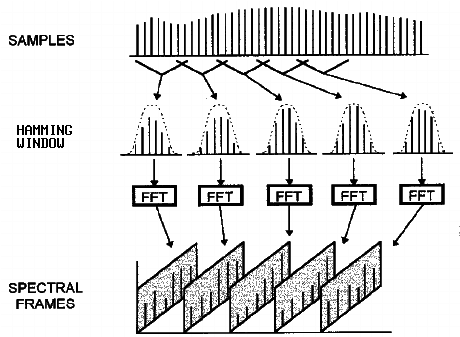
\includegraphics[width=\textwidth]{stft_pipe}
        \caption{Windowing is applied on overlapping segments\\ followed by FFT }
        \label{fig:STFT Pipe}
       \end{subfigure}
	    \begin{subfigure}[b]{0.4\textwidth}
        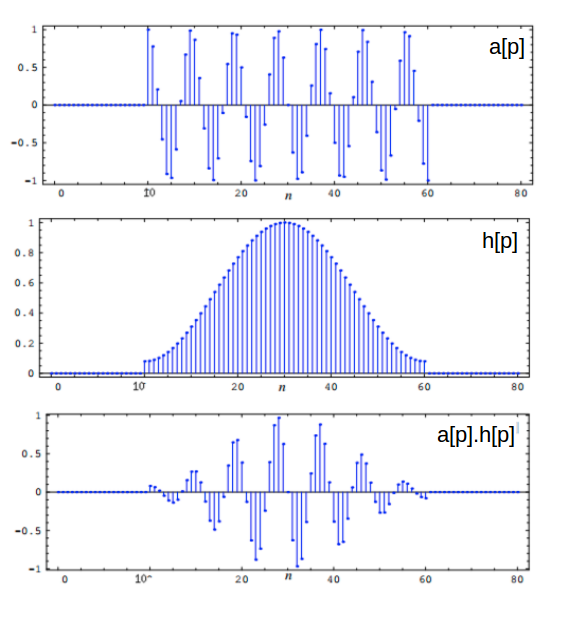
\includegraphics[width=\textwidth]{stft}
        \caption{
        Application of Hamming Window on \\a segment of input signal
        }
        \label{fig:Hamming Window}
       \end{subfigure}
       \caption{(a) Shows STFT Pipeline. (b) Shows the application of \\Window function}\label{fig:STFT}
\end{figure}
\bigskip

The discrete STFT (\textit{slow}) for $p^{th}$ frame of signal $\textbf{a}$ is obtained as,
\begin{equation}
\textbf{C}(p, \omega ) = \displaystyle\sum_{n=p.s}^{p.s + F}\textbf{a}(n)\textbf{h}(n-p.s)e^{-i \omega (n-p.s)}
\end{equation}
Where:
\begin{itemize}[label=]
    \setlength\itemsep{0em}
    \item $P$: is the number of spectral frames; $p \in [0,1..P-1]$ 
    \item $M$: is the dimension of discrete frequency space ; $\omega \in \mathbb{R}^{M}$
    \item $F$: is the frame length 
    \item $s$: is stride (or) hop-length for the next segment
    \item $\textbf{a} \in  \mathbb{R}^{N}$ ; $n \in [0,1...N-1]$
    \item $\textbf{h} \in  \mathbb{R}^{F}$
    \item $\omega \in  \mathbb{R}^{M}$
    \item $\textbf{C}$: is Fourier Coefficient Matrix ; $\textbf{C} : \mathbb{R}^{F.P} \rightarrow \mathbb{C}^{M \times P}$
\end{itemize}

\noindent Equation (2.11) can be seen as a \textbf{convolution} over the signal \textbf{a} with \textbf{W} which has finite support over the set $\left\{0,1..,F \right\}$ (more details in section ??)
\begin{equation}
\boxed
{
  \textbf{C}(p, \omega ) = \textbf{a}(n) \star \textbf{W}_{\omega}(n- \tau)
}
\end{equation}
Where:
\begin{itemize}[label=]
    \setlength\itemsep{0em}
    \item $ \tau$ = $p.s$
    \item $\textbf{W}_{\omega}(n- \tau)$ = $\textbf{h}(n- \tau )e^{-i \omega (n- \tau)}$
\end{itemize}
It is important to note that the coefficients $c_{\omega}$ may be complex valued. They are functions of the amplitude of corresponding sinusoidal component (see Appendix ??). But, to obtain useful metrics, we need to extract some physical quantity from the coefficients. This is where \textbf{Parseval's theorem} is used, which relates and time and frequency domain components in DFT as follows \cite{allen} :
\begin{equation}
{\|\textbf{c}\|}^2 \propto {\|\textbf{a}\|}^2
\end{equation}
If \textbf{a} represents amplitude in the time-domain, then as a consequence of Hook's law  on energy equation (see Appendix ??), we know that
\begin{equation}
Energy \propto amplitude^2
\end{equation}
Relating equation 2.11 and 2.12, it can be inferred that \textbf{square} of the Fourier coefficients is proportional to the energy distributed in the corresponding frequencies. This is called the \textbf{Power Spectrum (E)}. It is often motivating to use this representation because \textit{loudness} is proportional to \textit{energy}.
\begin{equation}
\textbf{E} = \textbf{C} \odot \textbf{C}
\end{equation}

\noindent As mentioned earlier, the frequencies in the considered range are  grouped into bins. It is useful to do so, not only to reduce dimension but also due to the aliasing effect of human auditory system. This is motivated by the human cochlea (an organ in the ear) which vibrates at different spots depending on the frequency of the incoming sounds. Depending on how frequencies are grouped, two different class of spectrograms are discussed.
  
\subsubsection{Mel Spectrogram}
\label{mel}

The \textit{mel-scale} was developed to express measured frequency in terms of psychological metrics (i.e perceived pitch). The mel-scale was developed
by experimenting with the human ears interpretation of a pitch. The experiment showed that the pitch is linearly perceived in the frequency range 0-1000 Hz. Above
1000 Hz, the scale becomes logarithmic. There are several formulae to convert Hertz to mel. A popularly used formula is noted in \cite{speech}
\begin{equation}
\omega_{m} = 2595log_{10}\bigg(1+\frac{ \omega }{700}\bigg)
\end{equation}
Where $\omega$ is the frequency in Hertz. In a mel spectrogram, the frequencies and converted to mels and then grouped into mel-spaced bins. This is done by multiplying the spectrum with some \textbf{filter bank ($\textbf{M}_{\omega_{m}}$)}. For details about computation of mel-filter banks, refer \cite{mel}. Each filter bank is centered at a specific frequency. Hence, to compute R mel bins, we need R mel-filter banks. 
\begin{equation}
\textbf{Mel}(p,\omega_{m}) = \displaystyle\sum_{ \omega = 0}^{M}\textbf{Y}(p, \omega)\textbf{M}_{\omega_{m}}(\omega)
\end{equation}
Where:
\begin{itemize}[label=]
    \setlength\itemsep{0em}
    \item $\textbf{Y}$ = $f(\textbf{C})$
    \item $\omega_{m}$ = mel frequency
\end{itemize}    
When the function $f$ is an defined by equation (2.15), we get \textbf{mel power spectrogram}
\bigskip

\noindent We can re-write equation (2.17) as, 
\begin{equation}
\textbf{Mel}(p,\omega_{m}) = \displaystyle\sum_{k=p.M}^{p.M + K}\textbf{U}(k)\textbf{M}_{\omega_{m}}(k-p.M)
\end{equation}
Where:
\begin{itemize}[label=]
    \setlength\itemsep{0em}
    \item $P$: is the number of spectral frames; $p \in [0,1..P-1]$ 
    \item $M$: is the dimension of discrete frequency space ; $\omega = k-p.M \in \mathbb{R}^{M}$
    \item $K$ = $M.P$ and $k \in [0,1...K]$
    \item $\textbf{U}(k)$ = $\textbf{Y}(i,j)$ ; $i = floor(\frac{k}{M})$ ; $j = k-floor(\frac{Mk}{M-1})$
    \item $\textbf{Y} \in \mathbb{R}^{M \times P}$
    \item $\textbf{U} \in \mathbb{R}^{M.P}$
    \item $\omega_{m} \in  \mathbb{R}^{R}$
    \item $\textbf{Mel}$: is Mel Spectrum Matrix ; $\textbf{Mel} : \mathbb{R}^{M.P} \rightarrow \mathbb{R}^{R \times P}$
\end{itemize}

\noindent Hence, we can represent mel-spectrogram as \textbf{M-strided convolution} over \textit{flattened} $\textbf{Y}$ with mel filters $\textbf{M}_{\omega_{m}}$ (i.e, the frequency axis of $\textbf{C}$ is contracted with each mel-filte)r, 
\begin{equation}
\boxed
{
  \textbf{Mel}(p, \omega_{m} ) = \textbf{U}(k) \star \textbf{M}_{\omega_{m}}(k - p.M)
}
\end{equation}
  
\subsubsection{Chromagram}

This representation takes advantage of the periodic perception of pitch. Two pitches are perceived similar in "color" if they differ by one or several octaves apart. Chromagram groups such periodic perceptions into same coefficient (chroma). All pitches that belong to the same chroma are said to be from same pitch class. [TODO: How is this computed?]
\begin{figure}[h] 
\centering
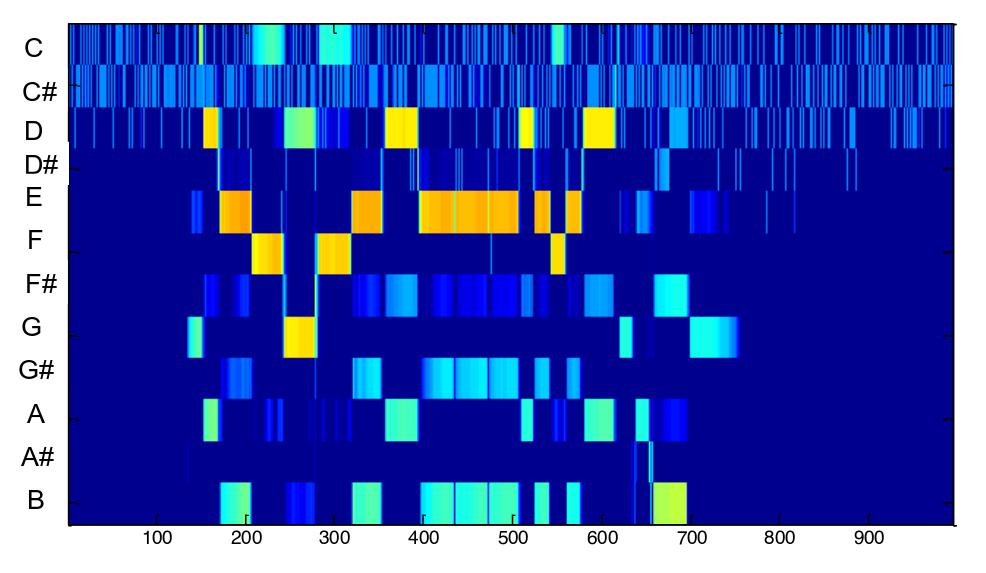
\includegraphics[width=0.5\textwidth]{chroma}
\caption{Chromagram of Western Pitch Scale}
 \label{fig:Chromagram}
 \end{figure}
\FloatBarrier
\bigskip

\section{Dimensionality Reduction}
\label{dimension}
The objective of dimensionality reduction is to retain only the desirable characteristics of the representations presented in section 2.1. This is done because the representation ($\textbf{R}$) can be large for longer audio tracks (because number of frames $P$ depends on length of the audio). Reduction over a large frame at once can lead to loss of temporal information (i.e, change of variables across frames). Hence, dimensionality reduction is done hierarchically, sometimes by stacking combination of these techniques. We generalize the operations on input signal $\textbf{a}$ as follows,
\[
   \textbf{R} = Rep(\textbf{a}) \qquad Rep : \mathbb{R}^{N} \rightarrow \mathbb{R}^{R \times P}
\]
\[
   \textbf{X} = f(\textbf{R}) \qquad f : \mathbb{R}^{R \times P} \rightarrow \mathbb{R}^{S \times Q} 
\]
\[
   \textbf{Y} = D(\textbf{X}) \qquad D : \mathbb{R}^{S \times Q} \rightarrow \mathbb{R}^{T \times W} 
\] 

\noindent The representation operations defined in the previous section can be a part of the function $Rep$. Since dimension reductions can be stacked, $f$ represents the previous reductions applied. $Q$ and $W$ are number of frames as a result of hierarchical windowing operation shown in fig (2.3). For the first reduction however, $f$ does not exist and hence represented by conditional arrow (dotted). The output of reduction $\textbf{Y} \in \mathbb{R}^{T \times W}$ will then be the reduced representation ($T < S$ or $W < Q$). Depending on how the function $D$ is defined, we will classify the techniques into broad categories.
\begin{itemize}
  \item Reduction by \gls{basis} transformation
  \item Reduction by neural networks
  \item Reduction by clustering 
\end{itemize} 
\begin{figure}[h] 
\centering
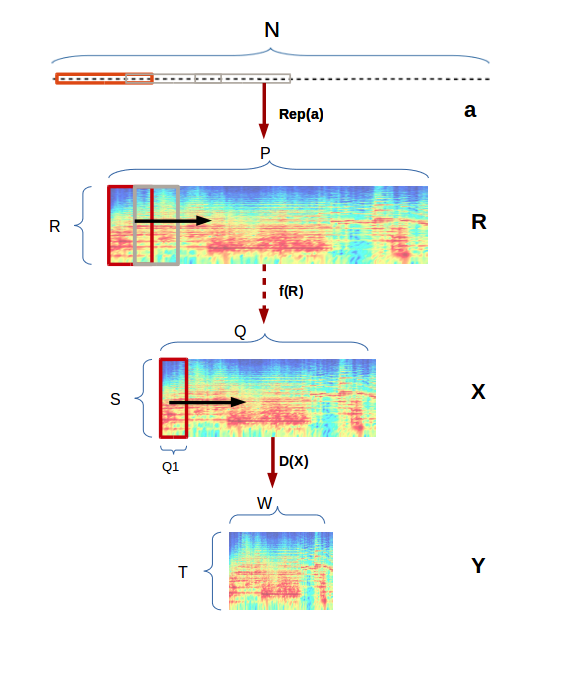
\includegraphics[width=0.5\textwidth]{dim_red}
\caption{Dimensionality Reduction Pipeline}
 \label{fig:Dimensionality Reduction}
 \end{figure}
\FloatBarrier
\bigskip

\subsection{Basis Transformations - PCA, MFCC}
\label{basis}

The \gls{basis} vectors are functions of the properties we want to encode. In equation (2.2), we used \gls{basis transformation} to represent the signal in frequency domain. Now we want to use the same concept, but for dimensionality reduction. In general terms, this is done by \textit{changing to a reduced basis}. That is, we need to find a   \gls{change of coordinates matrix} that will map the input to a basis system with lesser coordinates. 
\bigskip

\noindent The input frame $\textbf{X}_{w}$ is first operated with some window function $\textbf{w}$,
\[
  \textbf{z}_{w} = \{\textbf{X}_{w}\textbf{w} \quad | \quad \textbf{X}_{w} \in \mathbb{R}^{S \times J}, \textbf{w} \in \mathbb{R}^{J}, \textbf{z}_{w} \in \mathbb{R}^{S}\}
\]    
Now we have to compute $\textbf{y}_{w} \in \mathbb{R}^{T}$ which has least representation error with $\textbf{z}_{w} \in \mathbb{R}^{S}$ such that $T < S$. Let us say, $\textbf{z}_{w}$ can be written as a \gls{linear combination} of some \gls{basis} $\textbf{V} = [\textbf{v}_{1}, \textbf{v}_{2}, ..,\textbf{v}_{T}] \in \mathbb{R}^{S \times T}$ with coordinates $\textbf{y}_{w} = [y_{1}, y_{2},...,y_{T}]$. Then $\textbf{y}_{w}$ can be calculated by solving,
\[
\textbf{z}_{w} = \displaystyle\sum_{i=1}^{T}y_{i}\textbf{v}_{i} = \textbf{V}\textbf{y}_{w}
\]
\[
\textbf{y}_{w} = \textbf{V}^{-1}\textbf{z}_{w}
\]
Thus, the operator $D$ in equation (??) is,
\[
\textbf{Y} = D(\textbf{X}, \textbf{V})
\]
Therefore, dimension reduction through \gls{basis transformation} are those class of techniques where $D$ is a function of some invertible \gls{change of coordinates matrix} $\textbf{V}$. Now, depending on how $\textbf{V}$ is defined, some methods are discussed.

\subsubsection{Principal Component Analysis (PCA)}
The frequencies in the adjacent bins can be highly correlated and therefore contain redundant information. Principal component Analysis is a procedure to transform large number of correlated variables into smaller number of uncorrelated variables. This means, $\textbf{y}_{w}$ should be approximated only with basis vectors that account for large variance. Hence, in PCA based techniques, dimension reduction is done through \gls{basis} vectors of covariance matrix ($\bm{\Sigma}$). The coordinates of the resulting basis system are known as \textit{principal components}. The steps of this abstraction are enumerated,
\begin{enumerate}[label=(\alph*)]
\item The rows of $\textbf{X}$ are centred by their mean and covariance is computed as,
\[
   \bm{\Sigma} = \textbf{E}[(\textbf{X} - \textbf{E}[\textbf{X}])(\textbf{X} - \textbf{E}[\textbf{X}])^{T}] = \frac{1}{Q}\textbf{\^X}\textbf{\^X}^{T} \quad \in \mathbb{S}^{S \times S}
\]
\item The eigen values and eigen vectors of $\bm{\Sigma}$ are computed. At this point, we use the \gls{Orthogonal Eigenvector Decomposition Theorem} and infer that eigen vectors of symmetric matrix ($\bm{\Sigma}$) form an orthogonal basis in $\mathbb{R}^{S}$. 
\[
\bm{\Sigma} = \textbf{V}\bm{\Lambda}\textbf{V}^{T} \qquad \textbf{V} \in \mathbb{O}^{S \times S}, \quad \bm{\Lambda} \in \mathbb{D}^{S \times S}
\]

\item The eigen values represent the magnitude of variance for each frequency.  Hence, eigenvectors corresponding to large eigen values gives the coordinates corresponding to greater variance. So eigen vectors corresponding to top $T$ eigen values are retained, while ignoring coordinates of lower variance. The resulting \gls{change of coordinates matrix} is then $\textbf{\^V} \in \mathbb{O}^{S \times T}$
   
\item Since $\textbf{\^V}$ is orthogonal, $\textbf{\^{V}}^{-1} = \textbf{\^{V}}^{T}$, and we can compute $\textbf{y}_{w} = \textbf{\^{V}}^{T}\textbf{z}_{w}$

\end{enumerate}   



\begin{algorithm}
  \caption{$\textbf{Y}$ = PCA($\textbf{X}$)}\label{PCA}
  \begin{algorithmic}[1]
    \Statex \textbf{Input :} $\textbf{X} \in \mathbb{R}^{S \times Q}$
    \Statex \textbf{Output :} $\textbf{Y} \in \mathbb{R}^{T \times W}$
    \State  $W = \frac{Q}{Q_{s}}$
    \For{$i \in \{0,1,..,W\}$}
    \State $\textbf{X}_{s} = \textbf{X}[i.Q_{s}:(i+1).Q_{s}]$ \Comment{$\textbf{X}_{s} \in \mathbb{R}^{S \times Q_{s}}$}
      \State $\bm{\Sigma} = \frac{1}{Q_{s}}\textbf{X}_{s}\textbf{X}_{s}^{T}$ \Comment{$\bm{\Sigma} \in \mathbb{S}^{S \times S}$}
      \State $\textbf{V}, \bm{\lambda} = EIG(\bm{\Sigma}, T)$ \Comment{$\bm{\lambda} \in \mathbb{R}^{T}$ , $\textbf{V} \in \mathbb{O}^{S \times T}$}
      \State $\textbf{Y}[i] \leftarrow \textbf{V}^{T}\textbf{X}_{s}$
    \EndFor
  \end{algorithmic}
\end{algorithm}
\bigskip


\begin{algorithm}
  \caption{$\textbf{Y}$ = PCA WHITENING($\textbf{X}$) }\label{PCA_W}
  \begin{algorithmic}[1]
    \Statex \textbf{Input :} $\textbf{X} \in \mathbb{R}^{S \times Q}$
    \Statex \textbf{Output :} $\textbf{Y} \in \mathbb{R}^{T \times Q}$ \Comment{$W=Q$}
      \State $\bm{\Sigma} = \frac{1}{Q}\textbf{X}\textbf{X}^{T}$ \Comment{$\bm{\Sigma} \in \mathbb{S}^{S \times S}$}
      \State $\textbf{V}, \bm{\Lambda} = EIG(\bm{\Sigma}, T)$ \Comment{$\bm{\Lambda} \in \mathbb{D}^{T \times T}$ , $\textbf{V} \in \mathbb{O}^{S \times T}$}
      \State $\textbf{\^{X}} = ZERO\_MEAN(\textbf{X})$
      \State $\textbf{Y} \leftarrow \bm{\Lambda}^{-1}\textbf{V}^{T}\textbf{\^{X}}$
  \end{algorithmic}
\end{algorithm}
\bigskip


\begin{algorithm}
  \caption{$\textbf{Y}$ = MFCC($\textbf{a}$) }\label{MFCC}
  \begin{algorithmic}[1]
    \Statex \textbf{Input :} $\textbf{a} \in \mathbb{R}^{N}$
    \Statex \textbf{Output :} $\textbf{Y} \in \mathbb{R}^{S \times P}$ \Comment{$T=S$, $W=Q=T$}
    \State $\textbf{C} = STFT(\textbf{a})$ \Comment{$\textbf{C} \in \mathbb{C}^{M \times P}$}
    \State $\textbf{Y}_{r} = MODULUS(\textbf{C})$ \Comment{$\textbf{Y}_{r} \in \mathbb{R}^{M \times P}$}
    \State $\textbf{R} = MEL(\textbf{Y}_{r})$ \Comment{$\textbf{R} \in \mathbb{R}^{R \times P}$, $\textbf{X}=\textbf{R}$}
    \State $\textbf{R} \leftarrow ln(\textbf{R})$
    \State $\textbf{V} \leftarrow COSINE\_BASIS(R,S)$  \Comment{$\textbf{V} \in \mathbb{R}^{R \times S}$}
    \State $\textbf{Y} \leftarrow \textbf{V}^{T}\textbf{R}$
  \end{algorithmic}
\end{algorithm}
 
{\color{gray}
\subsection{Feature learning with stacked convolutions}
\label{stacked}

\subsubsection{Feature engineering Vs Feature Learning}
\label{feature}

\begin{figure}[h] 
\centering
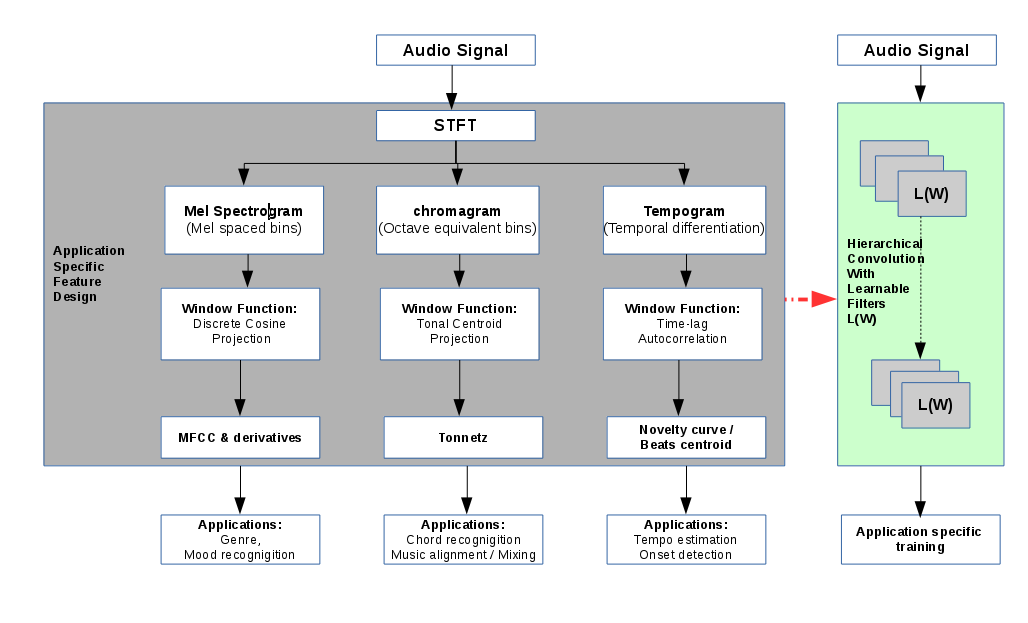
\includegraphics[width=0.95\textwidth]{dnn_motivation}
\caption{Motivation for deep architectures}
 \label{fig:deep learning}
 \end{figure}
\FloatBarrier
\bigskip

\section{Temporal pooling}
\label{temporal}
\subsection{Clustering}
\label{clustering}
\subsection{Recurrent Neural Networks}
\label{rnn}

\section{Training}
\label{training}
}
